\section{Headwise Analysis of Local/Retrieval Patterns and Retrieval Sparsity}
\label{appd:headwise}

In this section, we analyze the distribution and properties of different head patterns in the two models used in our experiments, namely Qwen3-Coder-30B-A3B and Qwen3-30B-A3B-Think, to better understand their multi-head attention behaviors.

\subsection{Headwise Distribution.}
\label{appd:distribution}

In this section, we analyze the distribution of retrieval scores across all query heads in Qwen3-Coder-30B-A3B and Qwen3-30B-A3B-Think.

\noindent\textbf{Retrieval score distribution.}
Figure~\ref{fig:headwise_attnmap} presents the per-head retrieval score heatmaps for both models. We make the following observations:

\begin{itemize}[leftmargin=*, itemindent=0pt]
    \item \emph{Heads with strong retrieval ability are relatively few.} Most query heads receive only small retrieval scores, indicating limited long-range recall ability, while only a relatively small subset of heads consistently exhibits strong retrieval behavior. This suggests that the capacity for long-range token recall is concentrated in a minority of heads, whereas the majority primarily rely on local context or sink tokens for information processing.

    \item \emph{Retrieval heads concentrate in later layers.} High-scoring retrieval heads are distributed highly unevenly across layers, appearing almost exclusively in the latter half of the model. This is consistent with the layerwise computation pattern of LLMs: early layers are primarily responsible for local contextualization, where token representations are still evolving; later layers produce more stable, semantically rich representations that provide the necessary foundation for reliable long-range token retrieval~\citep{ghandeharioun2024patchscopes}.

    \item \emph{Head behavior is highly stable and input-agnostic.} The retrieval scores of individual heads remain highly consistent across different input documents, confirming our assumption in Section~\ref{sec:offline_calibration} that running offline calibration on a single long sequence is sufficient to robustly partition all query heads into retrieval and local sets.
\end{itemize}

\paragraph{Comparison across models.}
Qwen3-30B-A3B-Think, as a reasoning-specialized model, exhibits a head distribution pattern largely consistent with Qwen3-Coder-30B-A3B: only a relatively small subset of heads shows strong retrieval ability, and these heads are likewise concentrated in the later layers. This suggests that head specialization is a general intrinsic property of pretrained LLMs, rather than an artifact of a specific task or model architecture.

\begin{figure}[t]
    \centering
    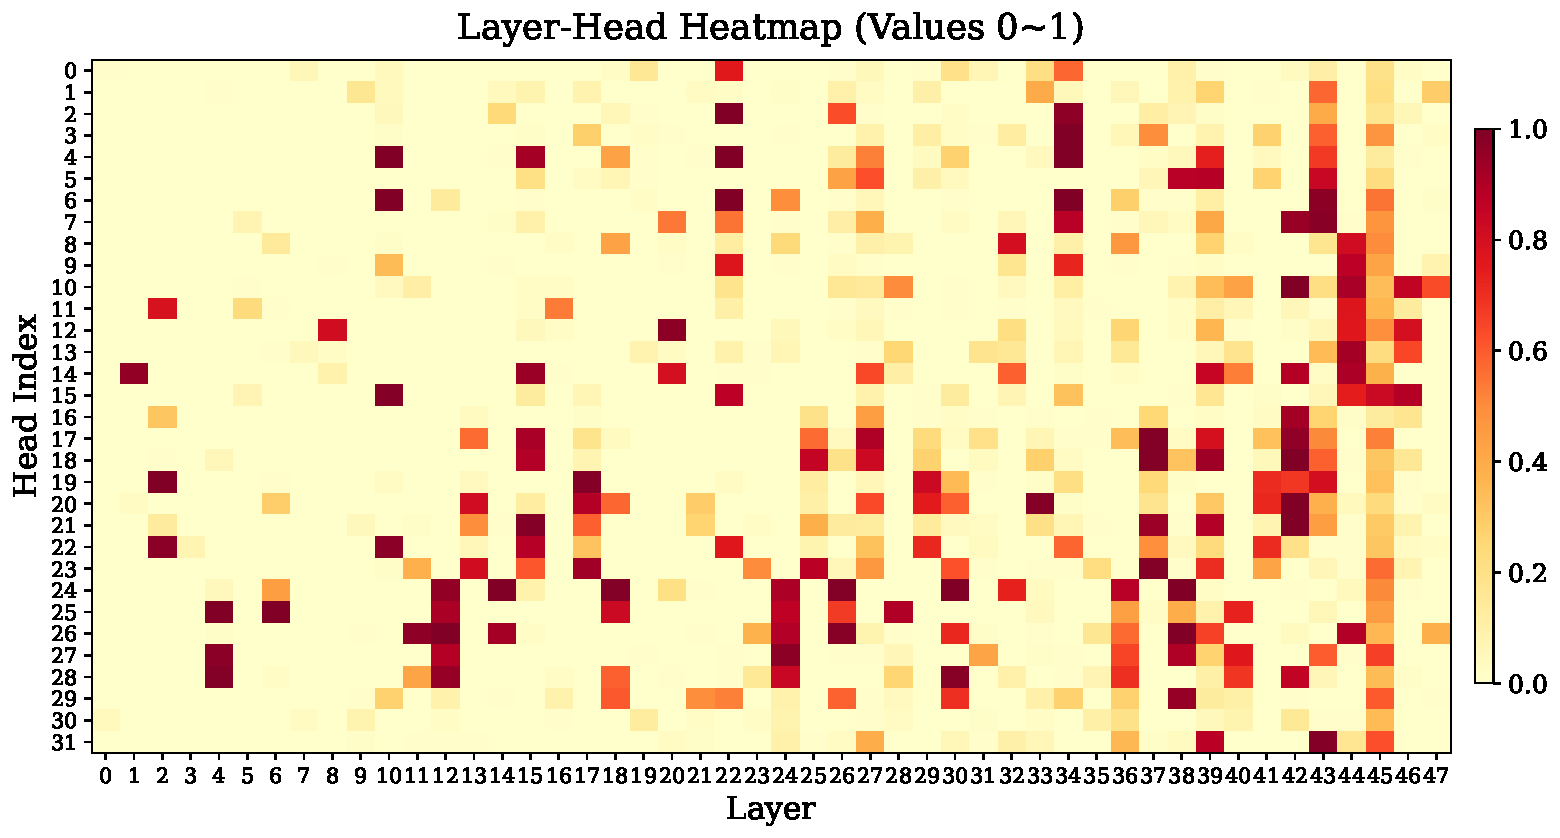
\includegraphics[width=\linewidth]{pic/appd/headwise_attnmap.pdf}
    \caption{Head-wise retrieval scores of all query heads in Qwen3-Coder-30B-A3B. A higher score indicates stronger long-range retrieval ability.}
    \label{fig:headwise_attnmap}
\end{figure}

\subsection{Diversity of Sparsity between Retrieval Heads.}
\label{appd:head_sparsity_diversity}

While Section~\ref{appd:distribution} characterizes the binary distinction between 
retrieval and local heads, we further analyze the token-level sparsity patterns 
within the retrieval head set $\mathcal{H}_\text{ret}$. Table~\ref{tab:appendix_headwise_topp_tokens} 
reports the number of tokens recalled by top-$p$ ($p = 0.9$) for three representative 
retrieval heads under different sequence lengths. The results reveal substantial diversity 
in sparsity behavior across individual retrieval heads:

\begin{itemize}[leftmargin=*, itemindent=0pt]
    \item \emph{Retrieval heads differ drastically in their token budgets.} 
    Even under the same top-$p$ threshold and the same input sequence, different 
    retrieval heads retain very different numbers of active tokens. For instance, 
    at 64K context length, \texttt{L43H31} retains only 21 tokens to cover 90\% 
    of attention mass, while \texttt{L24H25} requires 24{,}621 tokens to reach 
    the same coverage threshold---a gap of over three orders of magnitude. This 
    confirms that a single fixed top-$k$ budget cannot simultaneously serve all 
    retrieval heads: it would either over-retain tokens for highly concentrated 
    heads or under-retain for diffuse ones.

    \item \emph{Head-level sparsity patterns are consistent across context lengths.}
    Despite the absolute token counts scaling with sequence length, the relative 
    ordering of heads by sparsity remains stable. \texttt{L43H31} consistently 
    retains far fewer tokens than \texttt{L2H19} and \texttt{L24H25} across all 
    tested lengths (32K, 64K, and 128K), suggesting that each head's tendency 
    toward concentrated or diffuse retrieval is an intrinsic property of that head 
    rather than a transient artifact of a specific input.

    \item \emph{Sparsity diversity motivates per-head dynamic thresholding.}
    The stark contrast between heads such as \texttt{L43H31} (highly concentrated) 
    and \texttt{L24H25} (broadly diffuse) highlights why our top-$p$ mechanism 
    is essential. By applying an independent, query-aware threshold to each head, 
    \name naturally accommodates this diversity: concentrated heads are served 
    with minimal token budgets, while diffuse heads expand their active sets only 
    when necessary. This per-head adaptivity is precisely what static top-$k$ 
    methods fundamentally cannot provide.
\end{itemize}

\begin{table}[ht]
    \centering
    \small
    \caption{Number of recalled tokens selected by top-$p$ ($p=0.9$) for representative retrieval heads under different sequence lengths.}
    \label{tab:appendix_headwise_topp_tokens}
    \begin{tabular}{lccc}
        \toprule
        \textbf{Retrieval Head} & \textbf{32K} & \textbf{64K} & \textbf{128K} \\
        \midrule
        L2 H19  & 4540 & 10468 & 9858 \\
        L24 H25 & 13836 & 24621 & 39614 \\
        L43 H31 & 55 & 21 & 42 \\
        \bottomrule
    \end{tabular}
\end{table}

\section{Ablations on \name Design Choices}
\label{appd:ablation}

We conduct ablation studies on several key design settings in \name.

\subsection{Ablation on Retrieval Head Ratio}

We compare two retrieval-head ratios in \name, namely 15\% and 30\%, on representative subcategories from MMLU-PRO and RULER.

\begin{table}[ht]
    \centering
    \small
    \caption{Ablation on retrieval-head ratio over MMLU-PRO subcategories.}
    \label{tab:appendix_mmlupro_ratio}
    \begin{tabular}{lcc}
        \toprule
        \textbf{MMLU-PRO Subcategory} & \textbf{\name (15\%)} & \textbf{\name (30\%)} \\
        \midrule
        Biology & 86.0 & 85.8 \\
        Computer Science & 76.8 & 76.8 \\
        History & 56.1 & 56.1 \\
        Math & 88.2 & 88.2 \\
        Philosophy & 59.1 & 59.0 \\
        \bottomrule
    \end{tabular}
\end{table}

\begin{table}[ht]
    \centering
    \small
    \caption{Ablation on retrieval-head ratio over RULER sub-benchmarks.}
    \label{tab:appendix_ruler_ratio}
    \begin{tabular}{lcc}
        \toprule
        \textbf{RULER 64K} & \textbf{\name (15\%)} & \textbf{\name (30\%)} \\
        \midrule
        FWE & 81.7 & 81.4 \\
        HotPot & 62.8 & 62.6 \\
        multi-Q & 99.7 & 99.7 \\
        multi-K & 98.8 & 98.6 \\
        niah-S & 99.9 & 99.9 \\
        \bottomrule
    \end{tabular}
\end{table}

\begin{table}[ht]
    \centering
    \normalsize
    \setlength{\tabcolsep}{6pt}
    \renewcommand{\arraystretch}{1.10}
    \caption{Benchmarks with 15\% vs. 10\% retrieval-head ratios.}
    \label{tab:appendix_ratio_small}
    \begin{tabular}{lcc}
        \toprule
        \textbf{Benchmark} & \textbf{15\%} & \textbf{10\%} \\
        \midrule
        MMLU-PRO Math & 88.2 & 79.3 \\
        MMLU-PRO CS & 76.8 & 70.2 \\
        RULER multi-K & 98.8 & 97.4 \\
        \bottomrule
    \end{tabular}
\end{table}

The results in Tables~\ref{tab:appendix_mmlupro_ratio},~\ref{tab:appendix_ruler_ratio}, and~\ref{tab:appendix_ratio_small} reveal a clear trade-off across different retrieval-head ratios. Increasing the ratio from 15\% to 30\% brings almost no accuracy improvement on either MMLU-PRO or RULER, while it directly reduces the overall sparsity and increases the training cost, since the first stage must optimize roughly twice as many low-dimensional projection parameters. In contrast, reducing the ratio further to 10\% causes a substantial accuracy drop on several representative benchmarks, indicating that the number of retrieval heads becomes insufficient to preserve robust long-range recall. Therefore, for the model used in our experiments, namely Qwen3-30B-A3B, a 15\% retrieval-head ratio provides the best balance between sparsity, training cost, and accuracy, and is thus the most practical design choice.

\subsection{Ablation on Low-dimension Size}
\label{appd:lowdim}


\begin{table}[ht]
    \centering
    \small
    \caption{Ablation on low-dimension size over representative benchmarks.}
    \label{tab:appendix_lowdim_accuracy}
    \begin{tabular}{lccc}
        \toprule
        \textbf{Benchmark} & \textbf{dim=4} & \textbf{dim=16} & \textbf{dim=32} \\
        \midrule
        MMLU-PRO Math & 89.1 & 88.2 & 88.2 \\
        MMLU-PRO CS & 76.9 & 76.8 & 76.8 \\
        RULER niah-S & 100 & 99.9 & 99.9 \\
        RULER HotPot & 63.0 & 62.8 & 62.7 \\
        \bottomrule
    \end{tabular}
\end{table}

% \noindent\textbf{Kernel Efficiency.}

\noindent\textbf{End-to-end Accuracy.} We compare different low-dimensional sizes in \name and study how the projection dimension affects both end-to-end task accuracy and the fitting quality of the low-dimensional relevance space. Specifically, we evaluate three representative settings, namely dim $=4$, dim $=16$, and dim $=32$, on a subset of representative benchmarks. Table~\ref{tab:appendix_lowdim_accuracy} summarizes the end-to-end accuracy results. We observe that dim $=16$ and dim $=32$ deliver nearly identical accuracy across all evaluated benchmarks. Since increasing the dimension from 16 to 32 doubles the number of trainable low-dimensional projection parameters, this result suggests that dim $=16$ is already sufficient to capture the attention distribution of retrieval heads accurately, and that further enlarging the projection space brings little practical benefit.

Interestingly, dim $=4$ yields the highest end-to-end accuracy in this comparison. However, this should not be interpreted as evidence that a smaller low-dimensional space provides a better approximation. Instead, Table~\ref{tab:appendix_l24h25_lowdim_topp_tokens} shows that dim $=4$ has substantially weaker fitting ability, which causes the top-$p$ selector to recall many more tokens in order to cover the same amount of attention mass. As a result, the actual sparsity becomes much lower under dim $=4$, and the corresponding accuracy improves because the sparse model behaves more similarly to a less aggressively pruned model.

\noindent\textbf{Fitting Ability of Low-dimension Space.} Table~\ref{tab:appendix_l24h25_lowdim_topp_tokens} reports the number of recalled tokens for retrieval head \texttt{L24H25} under different projection dimensions when using top-$p$ with $p=0.9$. The results show a clear trade-off between expressiveness and sparsity. When the projection dimension is too small, the compressed relevance space cannot faithfully model the full attention distribution, forcing the selector to retain substantially more tokens in order to recover the same amount of attention mass. This is exactly what happens at dimension 4, where the recalled token count rises sharply across all sequence lengths, indicating poor fitting ability and weak sparsity. Increasing the dimension to 16 dramatically improves the quality of the approximation and yields the smallest recalled-token budget overall, showing that this setting best captures the retrieval structure of the head while preserving high sparsity. Further increasing the dimension to 32 does not bring additional benefit; instead, it consistently requires more recalled tokens than dimension 16. This suggests that a moderately compact subspace is sufficient, and that a larger projection dimension may introduce unnecessary flexibility without improving token selection quality. Therefore, we choose dimension 16 as the default setting, since it achieves the best balance between fitting accuracy, sparsity, and computational efficiency.

\begin{table}[ht]
    \centering
    \small
    \caption{Number of recalled tokens for retrieval head \texttt{L24H25} under top-$p$ ($p=0.9$) with different input lengths and projection dimensions.}
    \label{tab:appendix_l24h25_lowdim_topp_tokens}
    \begin{tabular}{lccc}
        \toprule
        \textbf{Dimension} & \textbf{32K} & \textbf{64K} & \textbf{128K} \\
        \midrule
        4  & 25256 & 45280 & 89081 \\
        16 & 13771 & 25725 & 49133 \\
        32 & 15526 & 28464 & 54727 \\
        \bottomrule
    \end{tabular}
\end{table}

% \subsection{Ablation on Top-$k$ budget}



\section{Details of the Two-Stage Training Pipeline}
\label{appd:training}

In this section, we present the detailed procedure of our two-stage training pipeline and analyze the overall training workflow for Qwen3-Coder-30B-A3B.

\begin{table}[t]
    \centering
    \begin{minipage}[t]{0.49\linewidth}
        \centering
        \normalsize
        \setlength{\tabcolsep}{6pt}
        \renewcommand{\arraystretch}{1.10}
        \captionof{table}{Stage-1 training configuration.}
        \label{tab:appendix_stage1_settings}
        \begin{tabular}{lc}
            \toprule
            \multicolumn{2}{c}{\textbf{Training Settings}} \\
            \midrule
            max-lr & 1e-3 \\
            warmup-steps & 100 \\
            lr-scheduler & consine \\
            weight-decay & 0.01 \\
            max-grad-norm & 1.0 \\
            \bottomrule
        \end{tabular}
    \end{minipage}\hfill
    \begin{minipage}[t]{0.49\linewidth}
        \centering
        \normalsize
        \setlength{\tabcolsep}{6pt}
        \renewcommand{\arraystretch}{1.10}
        \captionof{table}{Stage-2 training configuration.}
        \label{tab:appendix_stage2_settings}
        \begin{tabular}{lc}
            \toprule
            \multicolumn{2}{c}{\textbf{Training Settings}} \\
            \midrule
            max-lr & 3e-6 \\
            warmup-steps & 200 \\
            lr-scheduler & constant \\
            weight-decay & 0.01 \\
            max-grad-norm & 1.0 \\
            global-batch-size & 8 \\
            micro-batch-size & 1 \\
            \bottomrule
        \end{tabular}
    \end{minipage}
\end{table}

\subsection{Details of Low-dimension Projection Training}
\label{appd:train_stage_1}

For Qwen3-Coder-30B-A3B, the total number of query heads is 1536, with head dimension $d_h=128$. After offline calibration, we select the top 210 heads with the highest retrieval scores as retrieval heads, corresponding to roughly 15\% of all heads. For stage-1 training, we construct the training set by sampling 8,000 sequences from the open-source FineWeb dataset, each with a length between 32K and 80K tokens. For each retrieval head, our objective is to align the original attention-score distribution with the compressed attention-score distribution, while training only the low-dimensional query/key projection parameters. Under our setting, each head introduces $2 \times 128 \times 16 = 4096$ trainable parameters, corresponding to the query and key projections with head dimension 128 and low dimension 16. Therefore, the total number of trainable parameters in stage 1 is $210 \times 4096 \approx 8.6 \times 10^5$, i.e., about 840K parameters in total.

The training settings are summarized in Table~\ref{tab:appendix_stage1_settings}. Specifically, the learning rate is linearly warmed up from 0 to the peak value of $10^{-3}$ over the first 100 steps, and then decayed with a cosine annealing schedule. As shown in Figure~\ref{fig:stage1_indexer_loss}, the training loss of Layer 24 Head 25 already converges well within about 600 steps, and we observe highly similar convergence behavior for the other retrieval heads. Since each training sequence contains 48K tokens on average, the total token budget of this stage is approximately $48\mathrm{K} \times 600 \simeq 30\mathrm{M}$ tokens.


\begin{figure}[ht]
    \centering
    \begin{subfigure}[t]{0.49\linewidth}
        \centering
        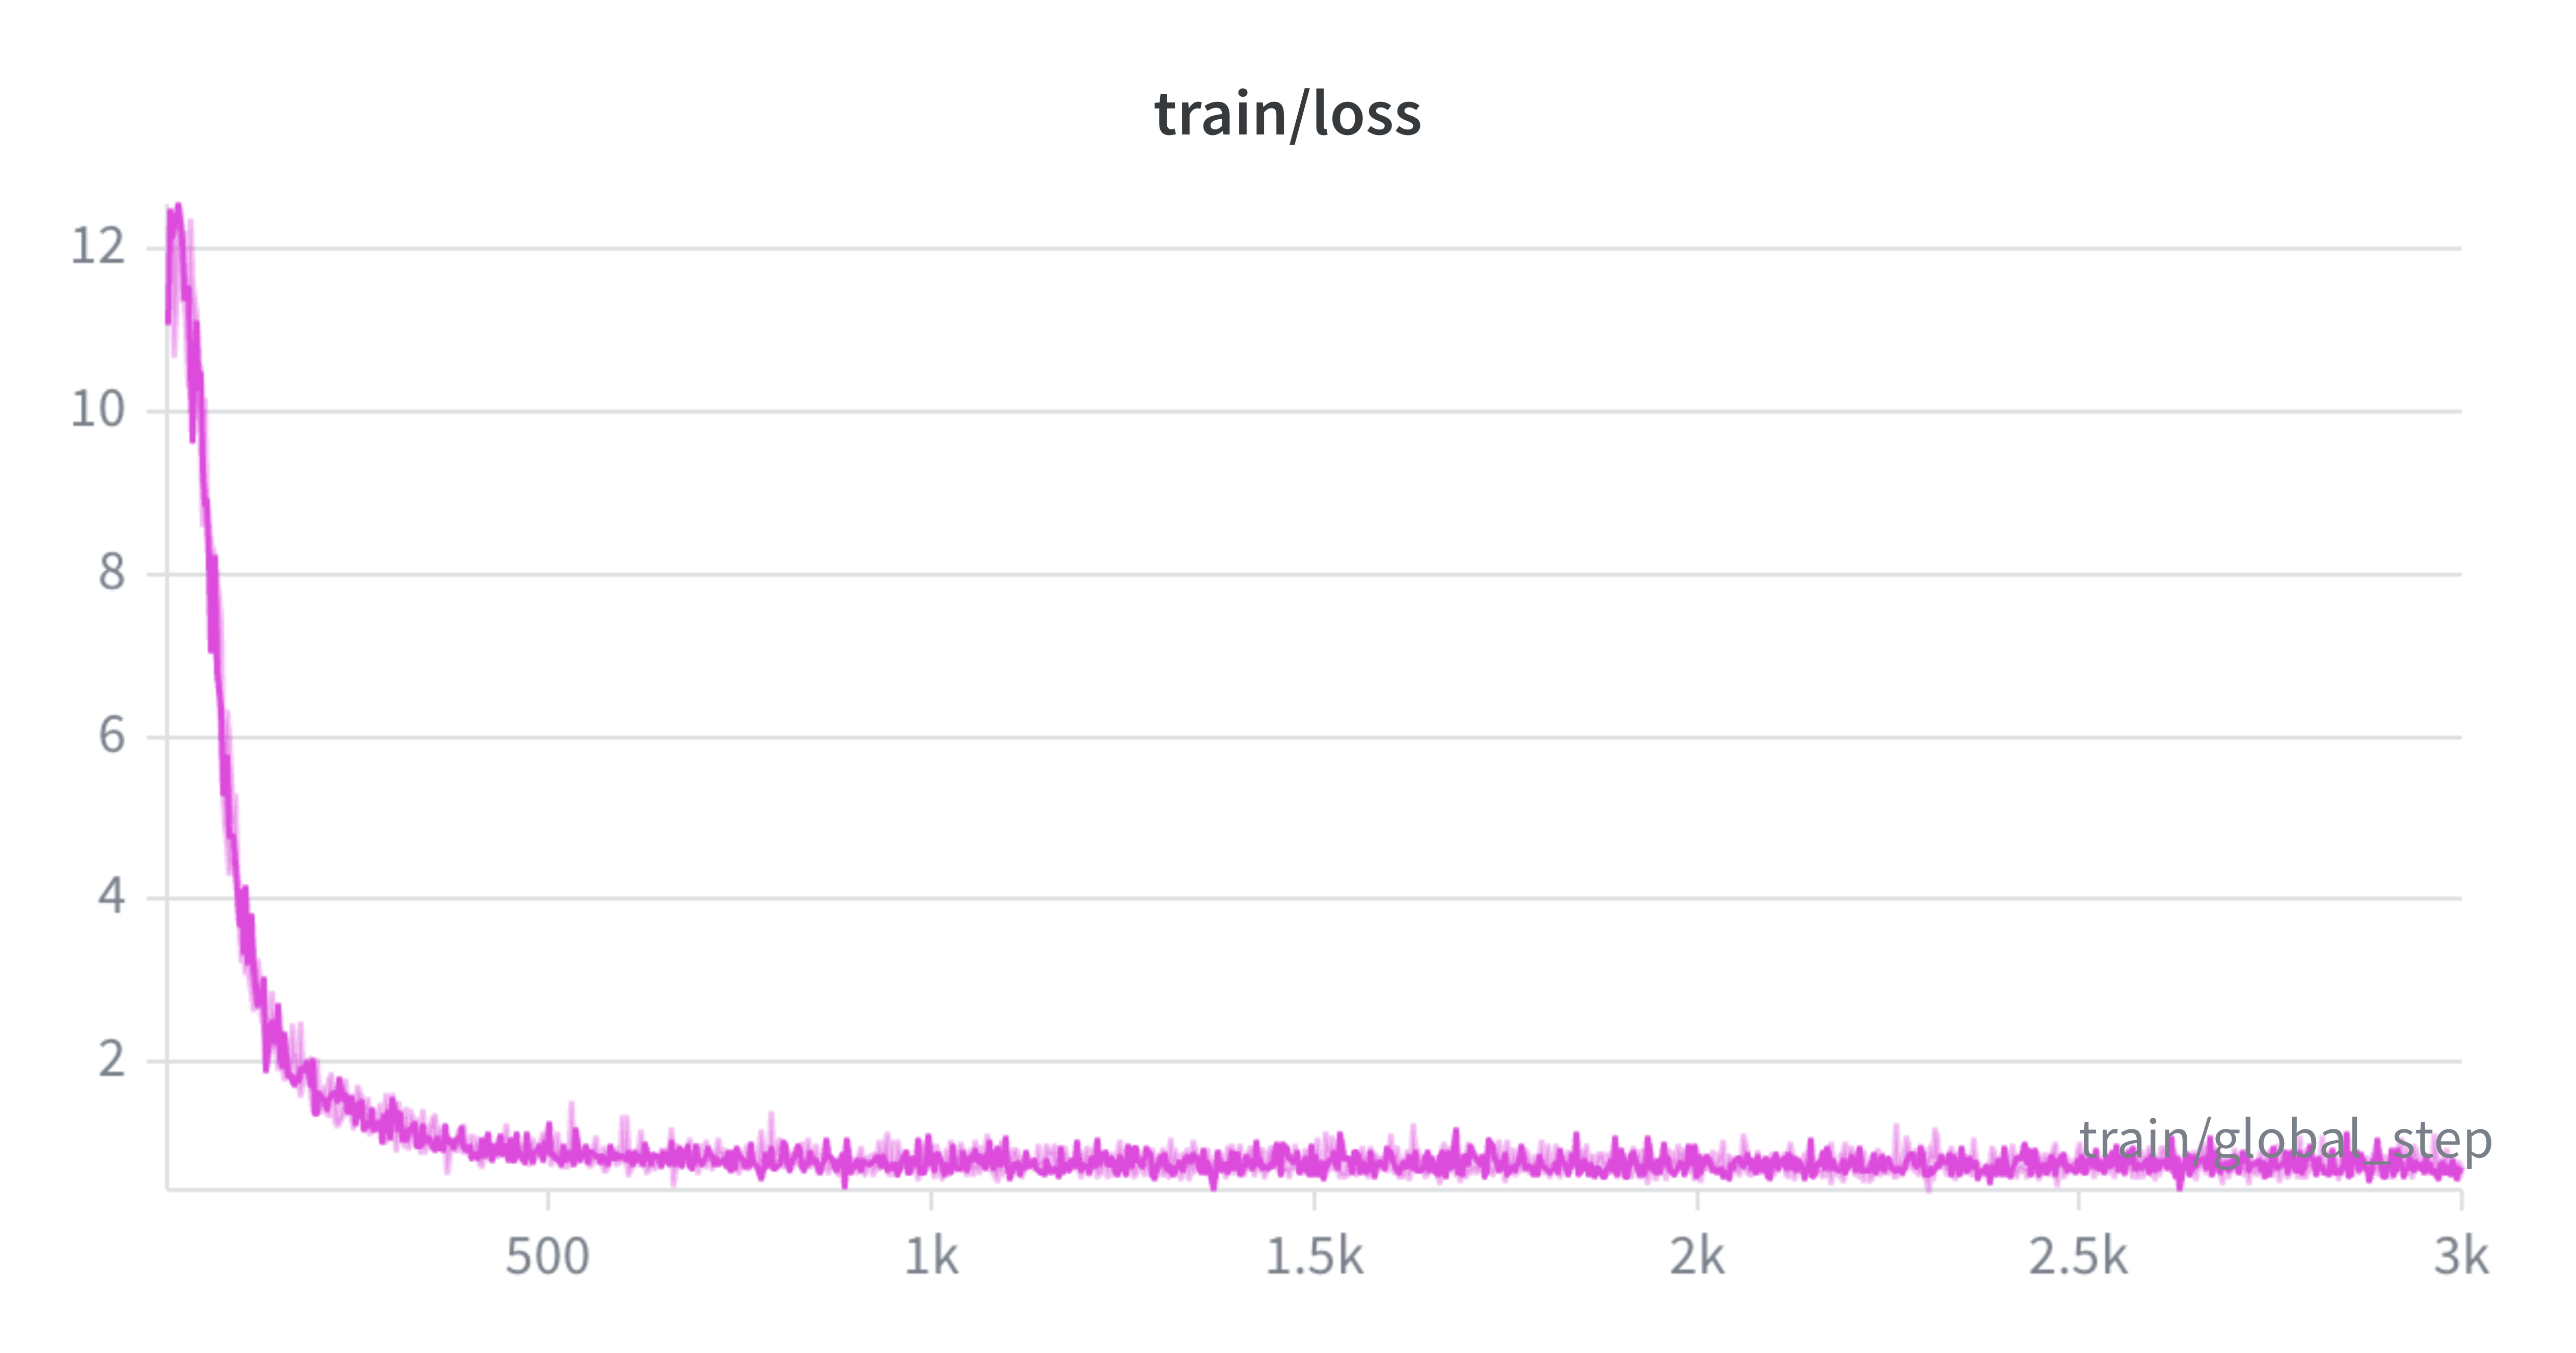
\includegraphics[width=\linewidth]{pic/appd/indexer-loss.png}
        \caption{Training loss curve of retrieval head L24H25 during stage-1 low-dimension projection training.}
        \label{fig:stage1_indexer_loss}
    \end{subfigure}\hfill
    \begin{subfigure}[t]{0.49\linewidth}
        \centering
        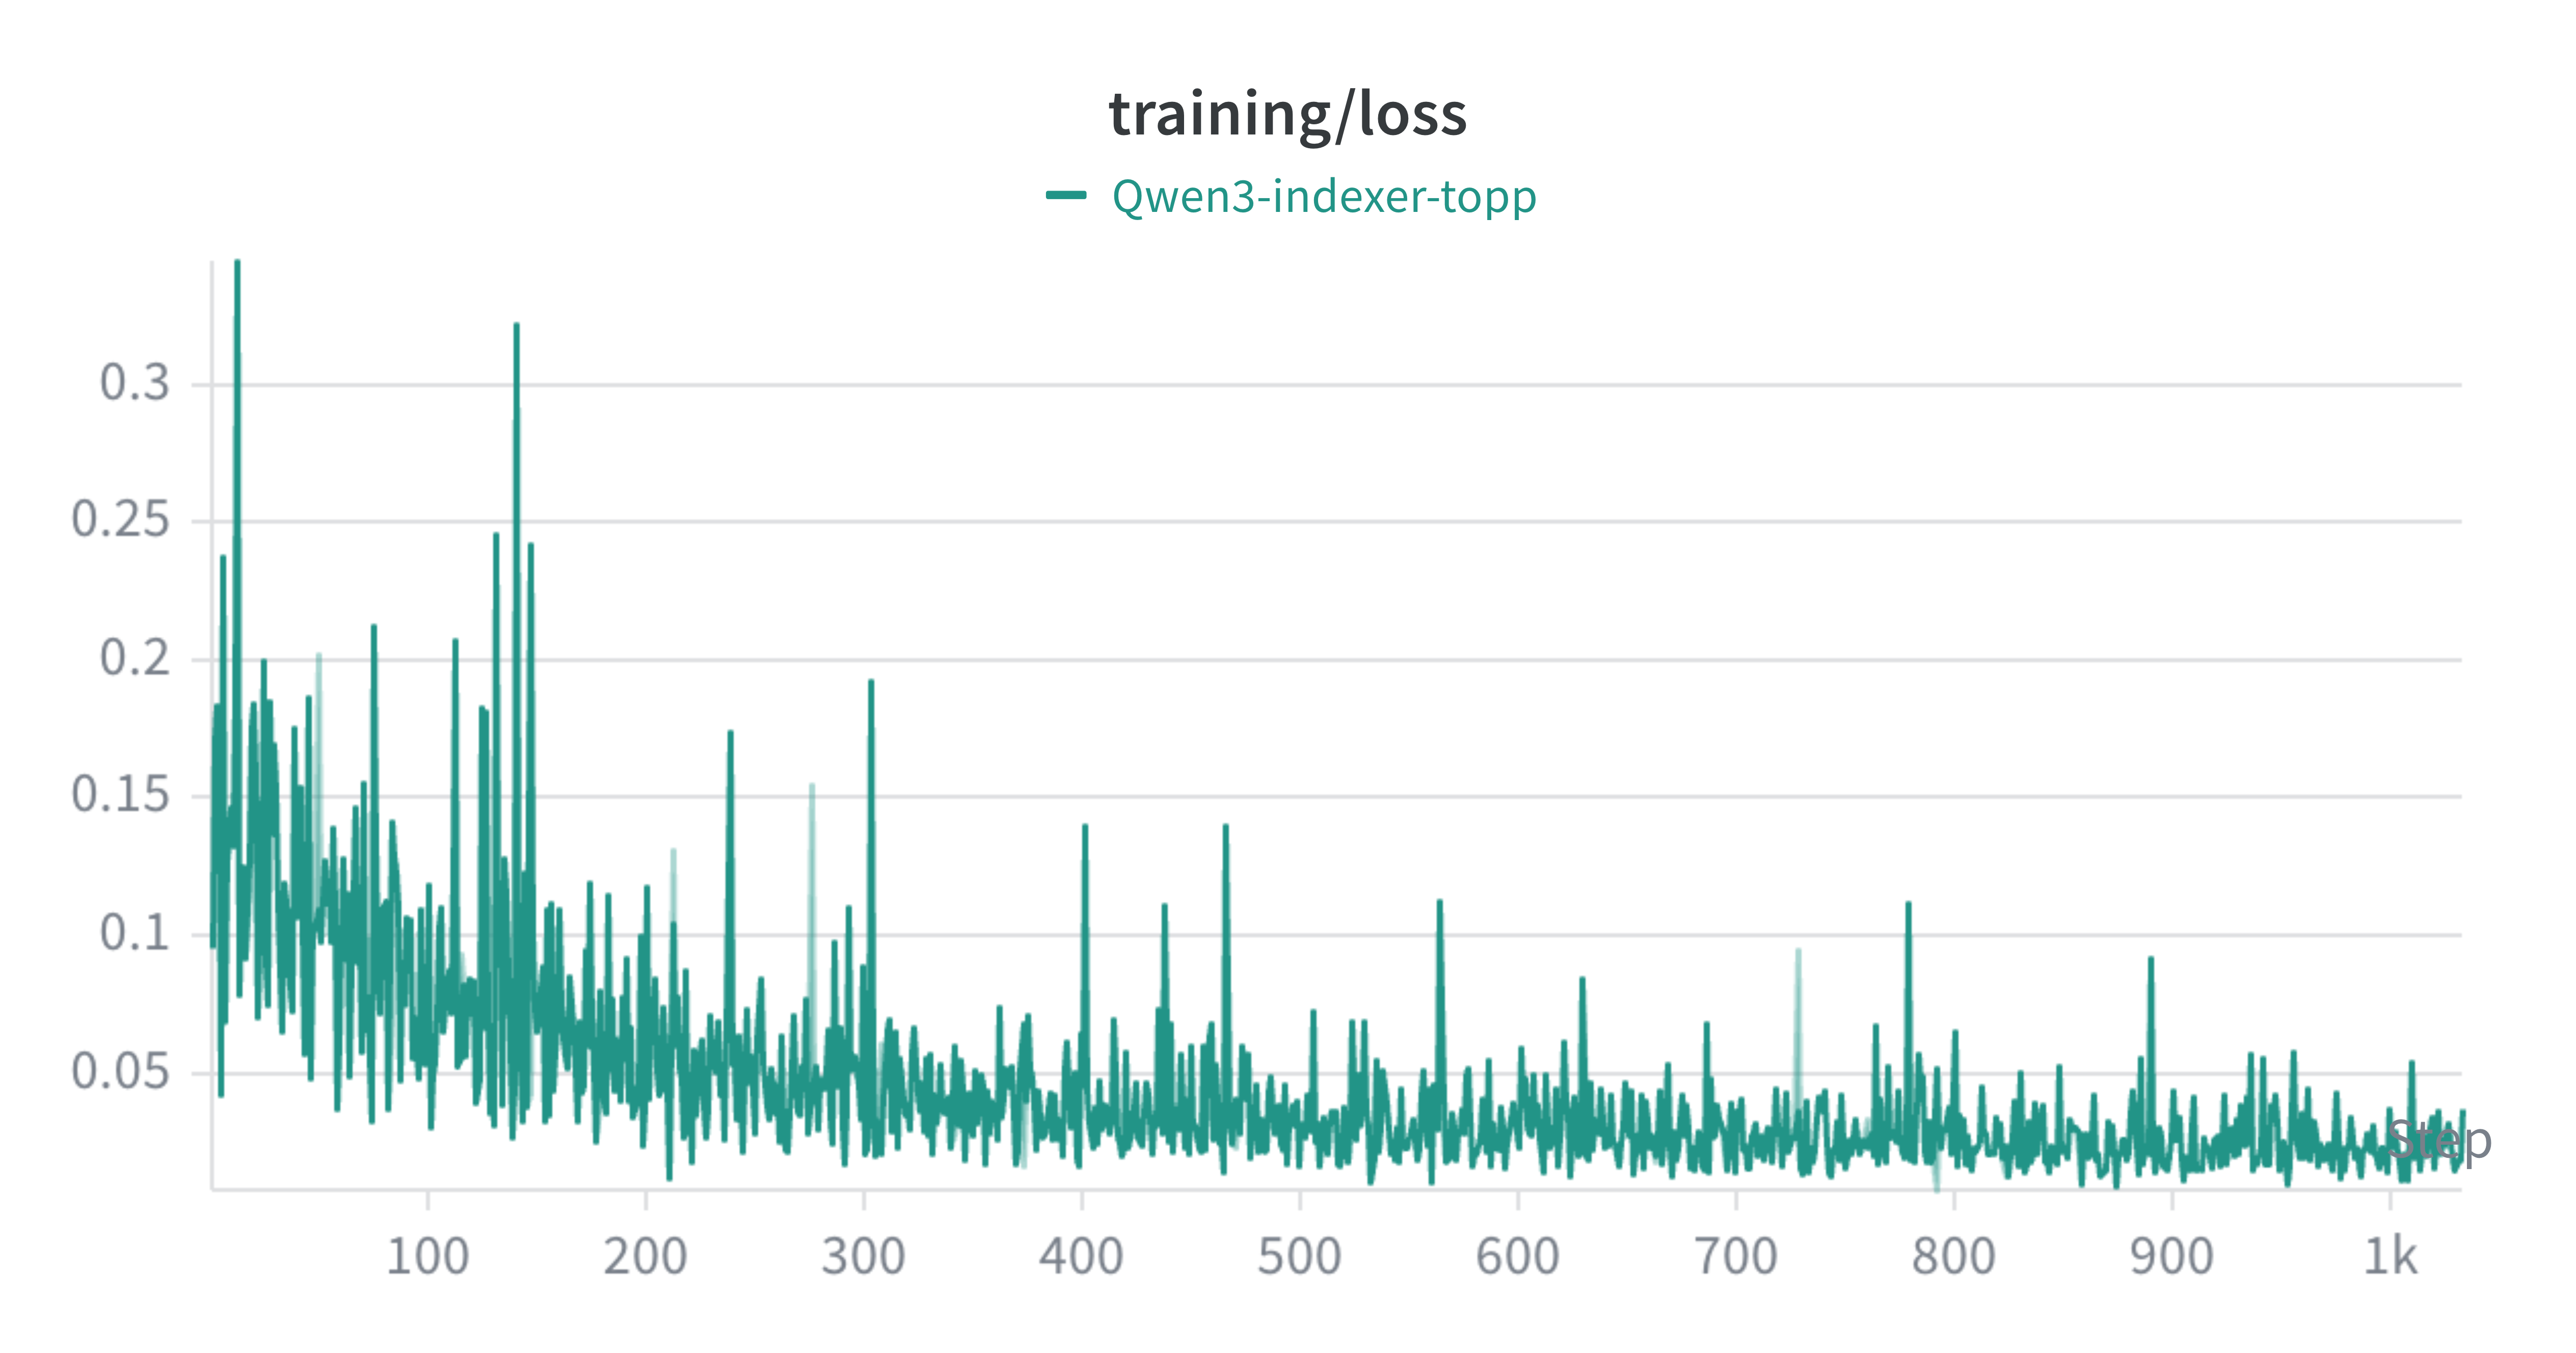
\includegraphics[width=\linewidth]{pic/appd/end2end.png}
        \caption{End-to-end training loss curve during stage-2 self-distillation.}
        \label{fig:stage2_end2end_loss}
    \end{subfigure}
    \caption{Training loss curves of the two-stage training pipeline.}
    \label{fig:two_stage_training_loss}
\end{figure}

\subsection{Details of End-to-End Self-distillation Training}
\label{appd:train_stage_2}

For stage-2 training, we sample 8,000 long reasoning examples in dialogue format from Dolma 3 Longmimo Mix. Each sequence is longer than 32K tokens, the average sequence length is about 48K tokens, and the average number of training label tokens is about 300. We first run a forward pass on the original model over the entire training set, extract the top-10 next-token prediction logits at each position, and cache them as distillation targets. During training, we attach the low-dimensional parameters learned in stage 1 to the selected retrieval heads and keep these parameters frozen, while performing end-to-end optimization over the model weights. The objective of this stage is to align the logits of the sparse model with those of the original model before sparsification.

The training settings are summarized in Table~\ref{tab:appendix_stage2_settings}. In particular, we use a relatively small learning rate to avoid drifting away from the model's original capabilities during end-to-end finetuning. As shown in Figure~\ref{fig:stage2_end2end_loss}, the training loss of stage 2 converges within about 600 steps. The full training corpus contains roughly 180M tokens in total, while the actual number of label tokens involved in learning is only about 1.2M.


\section{Limitation} \label{appd:limitation}

Although \name achieves strong efficiency--accuracy trade-offs, it still has several limitations.

\begin{itemize}[leftmargin=*, itemindent=0pt]
    \item \emph{Dependence on stable head specialization.} Our method relies on the empirical observation that attention heads can be partitioned into retrieval and local groups through offline calibration. While this behavior is stable in the models we study, the quality of this partition may degrade for models with weaker head specialization or under substantial domain shift.

    \item \emph{Incomplete sparsification and limited evaluation scope.} In the current design, retrieval heads still use full dense attention during prefill. In addition, our experiments mainly focus on the Qwen3 family and on long-context and reasoning workloads, so broader validation on other architectures and domains is still needed.
\end{itemize}

We expect these limitations to be addressed by future work on more adaptive head routing, stronger prefill sparsification, and broader cross-model evaluation.

% \section{Societal Impacts} \label{appd:impacts}

% Our work improves the inference efficiency of long-context language models without introducing a new foundation model or a new dataset. Its societal impacts are therefore mainly indirect, through reducing the cost of deploying existing long-context models.

% On the positive side, better efficiency can reduce compute, latency, and energy usage, making long-context capabilities more accessible for research and practical applications such as long-document understanding and code assistance. On the negative side, lower serving cost may also modestly lower the barrier to deploying such models in sensitive settings or at larger scale, including applications that process private text.

% We do not release new personal data or high-risk generative assets in this work. We encourage downstream users to follow the safety, privacy, and licensing requirements of the underlying models and datasets when deploying \name.